\documentclass[tikz,border=6pt]{standalone}
\usepackage[T1]{fontenc}
\usepackage[utf8]{inputenc}
\usepackage{pgfplots}
\usepgfplotslibrary{groupplots}
\usetikzlibrary{calc}
\pgfplotsset{compat=1.18}
\begin{document}
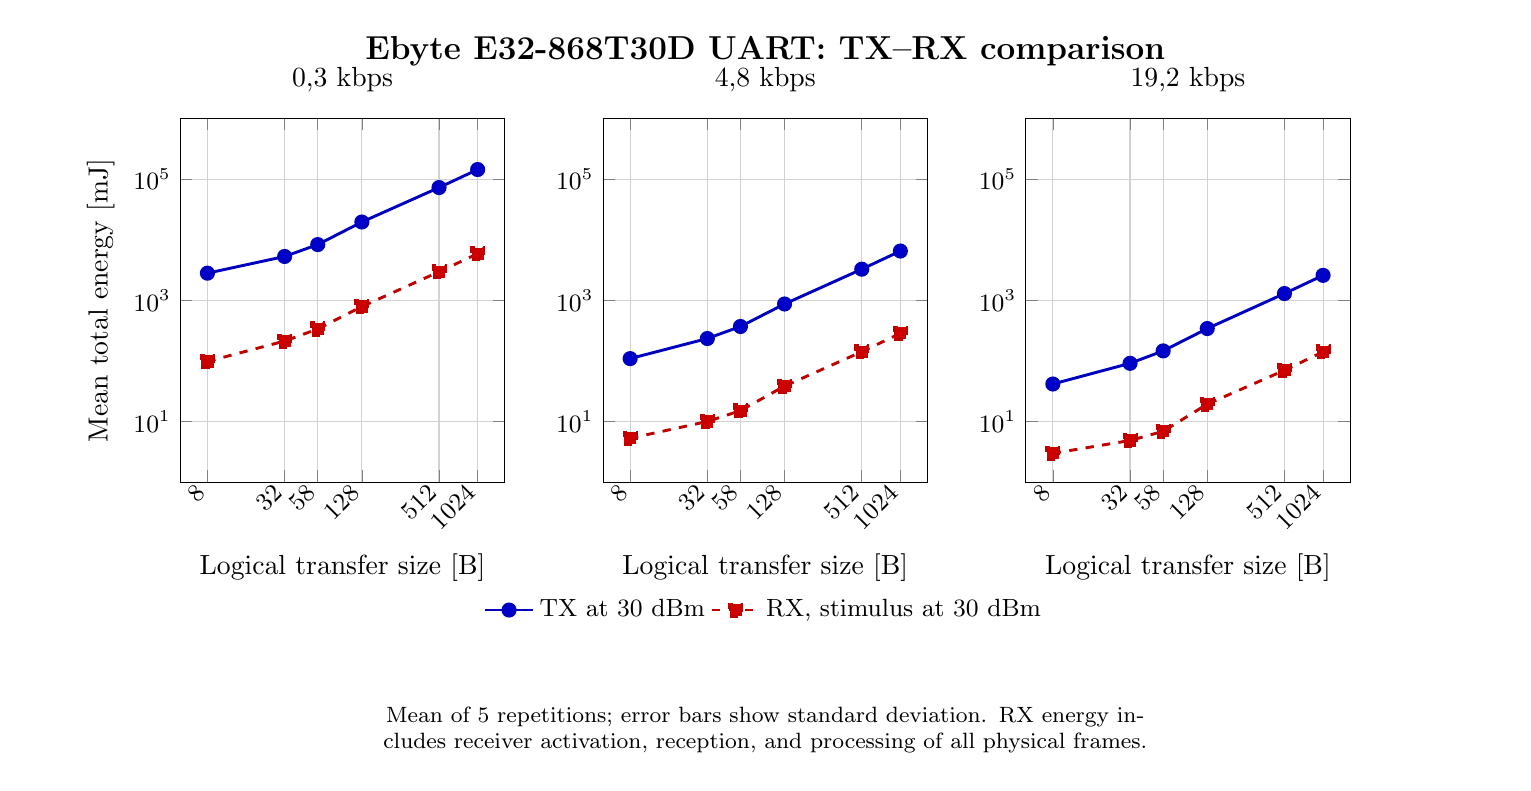
\begin{tikzpicture}
\begin{groupplot}[/pgf/number format/use comma,
  group style={group size=3 by 1, horizontal sep=1.25cm},
  width=5.7cm, height=6.2cm,
  xmode=log, log basis x={2}, ymode=log, log basis y={10},
  ymin=1, ymax=1000000,
  xtick={8,32,58,128,512,1024}, xticklabels={8,32,58,128,512,1024},
  x tick label style={rotate=45, anchor=east, font=\small},
  y tick label style={font=\small},
  grid=both, minor grid style={gray!15}, major grid style={gray!35},
  xlabel={Logical transfer size [B]},
  every axis plot/.append style={line width=1.05pt},
  error bars/error bar style={line width=0.35pt},
  legend style={font=\small, draw=none, fill=none, at={(0.5,-0.29)},
    anchor=north, legend columns=-1},
]
\nextgroupplot[title={0{,}3 kbps}, ylabel={Mean total energy [mJ]}]
\addplot+[color=blue!75!black, solid, mark=*, mark size=2.2pt,
  error bars/.cd, y dir=both, y explicit,
] coordinates {
  (8,2814.28226) +- (0,4.13387105)
  (32,5305.48879) +- (0,4.70177109)
  (58,8339.70933) +- (0,10.3552026)
  (128,19664.3831) +- (0,14.0746809)
  (512,72822.727) +- (0,39.2063401)
  (1024,144285.274) +- (0,439.556555)
};
\addplot+[color=red!75!black, dashed, mark=square*, mark size=2.2pt,
  error bars/.cd, y dir=both, y explicit,
] coordinates {
  (8,98.2826873) +- (0,0.219960975)
  (32,213.564188) +- (0,0.40068429)
  (58,337.724162) +- (0,0.83724591)
  (128,791.470694) +- (0,0.714825947)
  (512,2967.86515) +- (0,5.81465931)
  (1024,5910.5183) +- (0,2.70848665)
};
\nextgroupplot[title={4{,}8 kbps}]
\addplot+[color=blue!75!black, solid, mark=*, mark size=2.2pt,
  error bars/.cd, y dir=both, y explicit,
] coordinates {
  (8,109.657169) +- (0,0.0590503996)
  (32,235.08446) +- (0,0.204491425)
  (58,371.226943) +- (0,0.189004648)
  (128,872.800056) +- (0,0.814247858)
  (512,3275.17529) +- (0,3.78936838)
  (1024,6525.03387) +- (0,11.3160782)
};
\addlegendentry{TX at 30 dBm}
\addplot+[color=red!75!black, dashed, mark=square*, mark size=2.2pt,
  error bars/.cd, y dir=both, y explicit,
] coordinates {
  (8,5.30886837) +- (0,0.00234806533)
  (32,10.0426607) +- (0,0.00189900742)
  (58,15.1856378) +- (0,0.00818975858)
  (128,38.5651537) +- (0,0.0541144221)
  (512,142.39017) +- (0,0.0564326848)
  (1024,285.818114) +- (0,0.145554968)
};
\addlegendentry{RX, stimulus at 30 dBm}
\nextgroupplot[title={19{,}2 kbps}]
\addplot+[color=blue!75!black, solid, mark=*, mark size=2.2pt,
  error bars/.cd, y dir=both, y explicit,
] coordinates {
  (8,41.748603) +- (0,0.0361675683)
  (32,91.6482983) +- (0,0.033292413)
  (58,146.891371) +- (0,0.0511492973)
  (128,343.362814) +- (0,0.269087228)
  (512,1298.43098) +- (0,1.86862391)
  (1024,2590.62142) +- (0,2.57680654)
};
\addplot+[color=red!75!black, dashed, mark=square*, mark size=2.2pt,
  error bars/.cd, y dir=both, y explicit,
] coordinates {
  (8,2.99535784) +- (0,0.0162652666)
  (32,4.88444277) +- (0,0.00229513338)
  (58,6.92148966) +- (0,0.00355337462)
  (128,19.4580446) +- (0,0.00628137072)
  (512,70.3442722) +- (0,0.0607318438)
  (1024,141.64699) +- (0,0.0629022052)
};
\end{groupplot}
\node[font=\bfseries\large] at ($(group c2r1.north)+(0,0.85cm)$)
  {Ebyte E32-868T30D UART: TX--RX comparison};
\node[font=\footnotesize, align=center, text width=18.5cm]
  at ($(group c2r1.south)+(0,-3.15cm)$)
  {Mean of 5 repetitions; error bars show standard deviation. RX energy includes receiver activation, reception, and processing of all physical frames.};
\end{tikzpicture}
\end{document}
